\documentclass[twocolumn,showpacs,floatfix,longbibliography]{revtex4-1}
\usepackage{graphicx}
\usepackage{bm} % bold math
\usepackage{amssymb} % use this package to enable \nrightarrow command
\usepackage{amsmath} % use this package to enable \xrightarrow command
\usepackage{braket} % use for Dirac bra-kets : \rangle \labgle & \mid
\usepackage{natbib} % bibtex package
\usepackage{hyperref}


\begin{document}

\title{Skyrmion-induced bound states in a superconductor}

\author{Sergey S. Pershoguba$^{1}$}
\author{Sho Nakosai$^{1,2}$}
\author{Alexander V. Balatsky$^{1,3}$}
\affiliation{$^1$Nordita, Center for Quantum Materials, KTH Royal Institute of Technology, and Stockholm University, Roslagstullsbacken 23, S-106 91 Stockholm, Sweden}
\affiliation{$^2$Department of Applied Physics, University of Tokyo, Tokyo 113-8656, Japan}
\affiliation{$^3$Institute for Materials Science, Los Alamos National Laboratory, Los Alamos, New Mexico 87545, USA}

\date{\today}


\begin{abstract}
We consider a superconductor proximity coupled to a two-dimensional ferromagnet film with a skyrmion. Using the T-matrix calculations as well as numerical modeling we calculate the spin-polarized local density of states in the superconductor in the vicinity of the skyrmion. We find that the skyrmion bound states (SBS) are induced similar to the well-known Yu-Shiba-Rusinov (YSR) states. The wavefunction of SBS has a spatial  power-law decay. Therefore, in the presence of multiple skyrmions, superconductivity could facilitate an effective long-range interaction when the SBS wavefunctions, induced by different skyrmions, overlap.
\end{abstract}

\pacs{ }   

%%%%%%%%%%%%%%%%%%%%%%%%%%%%%%%%%%%%%%%%%%%%%%%%%%%%%%%%%%%%%%%%%%%%%%%%%%

\maketitle
%%%%%%%%%%%%%%%%%%%%%%%%%%%%%%%%%%%%%%%%%%%%%%%%%%%%%%%%%%%%%%%%%%%%%%%%%%%
\paragraph*{Introduction.---} \label{sec:intro}
%%%%%%%%%%%%%%%%%%%%%%%%%%%%%%%%%%%%%%%%%%%%%%%%%%%%%%%%%%%%%%%%%%%%%%%%%%%

Skyrmions, topological particle-like configurations of a continuous vector field, were originally proposed in the context of high-energy physics.  Nevertheless, it was suggested theoretically \cite{Bogdanov1989,Rossler2006} and recently observed experimentally \cite{Muhlbauer2009,Munzer2010,Yu2011,Heinze2011,Seki2012} that skyrmions exist in chiral ferromagnets in the presence of Dzyaloshinkii-Moriya interaction. Due to non-trivial topological properties, skyrmions manifest anomalous transport response to temperature gradients \cite{Jonietz2010} and electric field \cite{Neubauer2009,Zang2011,Saxena2013}. Recently, Hamburg group demonstrated a controllable writing and deleting of single skyrmions on the surface of PdFe bilayer \cite{Romming2013,Bergmann2014,Romming2015}. Coupling of magnetic films with skyrmions to novel materials holds a new promising avenue. For example, interplay of a magnetic skyrmion and a topological insulator was recently considered in Ref.~\cite{Hurst2015}. These developments show that skyrmions hold a great promise in applications such as spintronics, memory devices, etc \cite{Fert2013,Nagaosa2013}. 


In parallel, there has been an immense amount of interest recently in superconductor-ferromagnet (SC-FM) heterostructures aimed at engineering topological SC \cite{Alicea2012}. Discovery of the topological SC would entail existence of the Majorana edge modes, which would pave the way to realizing topological quantum computing \cite{Nayak2008}. So, motivated by the interest in skyrmions, on the one hand, and SC-FM heterostructures, on the other, we connect the two fields in the current work. Few works have considered skyrmions in the context of superconductivity. Reference~\cite{Garaud2011} studied the skyrmion-defects in the multiband superfluids and SCs. Paper \cite{Nakosai2013} discussed a possibility of realizing a topological SC using a skyrmionic lattice. The Josephson current through a magnetic skyrmion structure was considered in Ref.~\cite{Yokoyama2015}. However, none of the papers considered the conceptually simplest case of interaction between a single skyrmion and SC, which is the subject of the discussion below.

%%%%%%%%%%%%%%%%%%%%%%%%%%%%%%%%%%%%%%%%%%%%%%%%%%%%%%%%%%%%%%%%%%%%%%%%%%%
\begin{figure} \centering
(a) 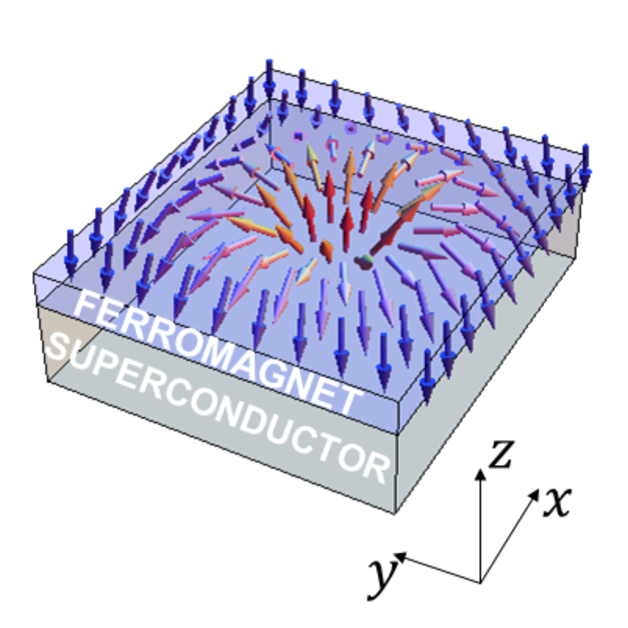
\includegraphics[width=0.4\linewidth]{SkyrmA}  
(b) 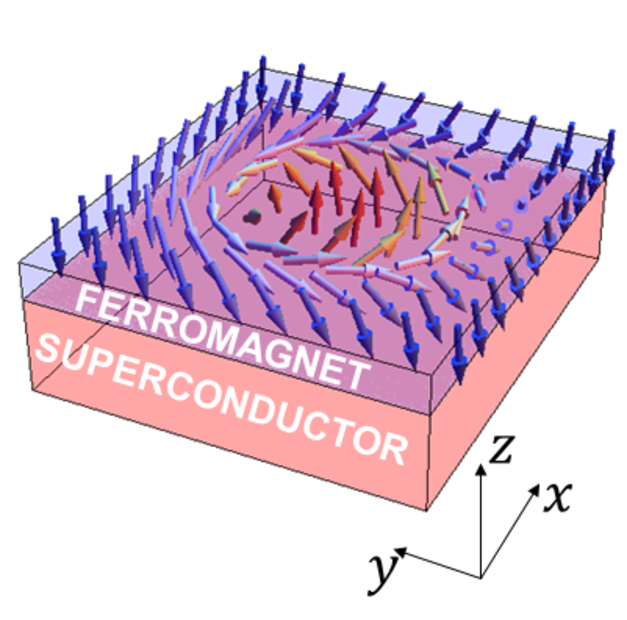
\includegraphics[width=0.4\linewidth]{SkyrmB} \\
(c) 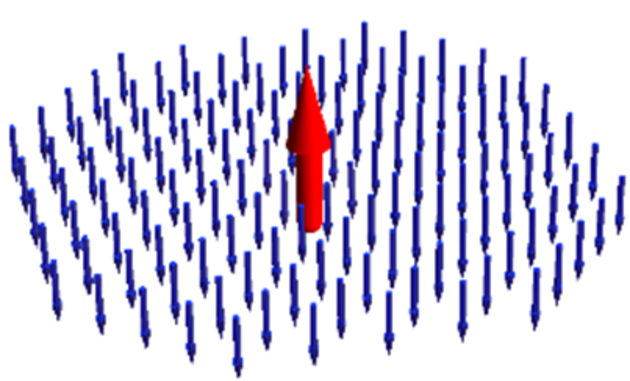
\includegraphics[width=0.4\linewidth]{fig1c}
\caption{(Color online.) (a,b) System under consideration: ferromagnetic (FM) film with a skyrmion proximity coupled to a superconductor (SC). (a) N\'eel-type (hedgehog) skyrmion.  (b) Bloch-type (spiral) skyrmion. (c) Sketch of an approximation of a skyrmion as a local magnetic moment floating in a ``ferromagnetic sea''.} \label{fig:skyrmion}
\end{figure}
%%%%%%%%%%%%%%%%%%%%%%%%%%%%%%%%%%%%%%%%%%%%%%%%%%%%%%%%%%%%%%%%%%%%%%%%%%



%%%%%%%%%%%%%%%%%%%%%%%%%%%%%%%%%%%%%%%%%%%%%%%%%%%%%%%%%%%%%%%%%%%%%%%%%%%
\begin{figure} \centering
%	(a)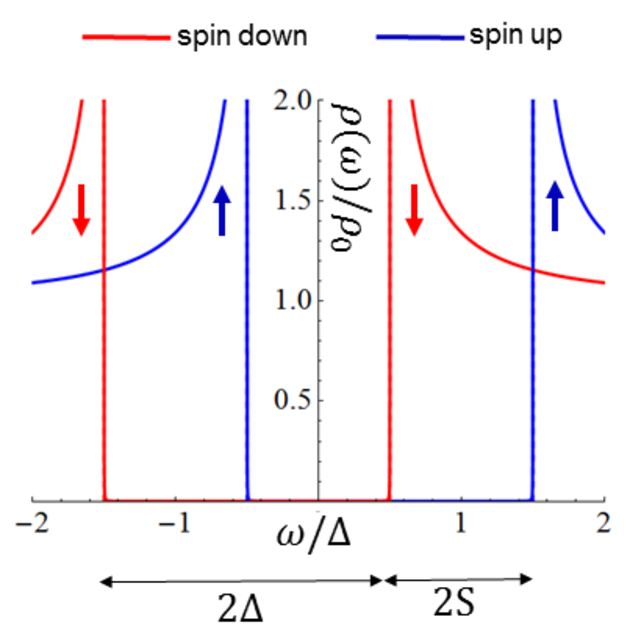
\includegraphics[width=0.25\linewidth]{LDOSa} \hspace{0.1cm}
	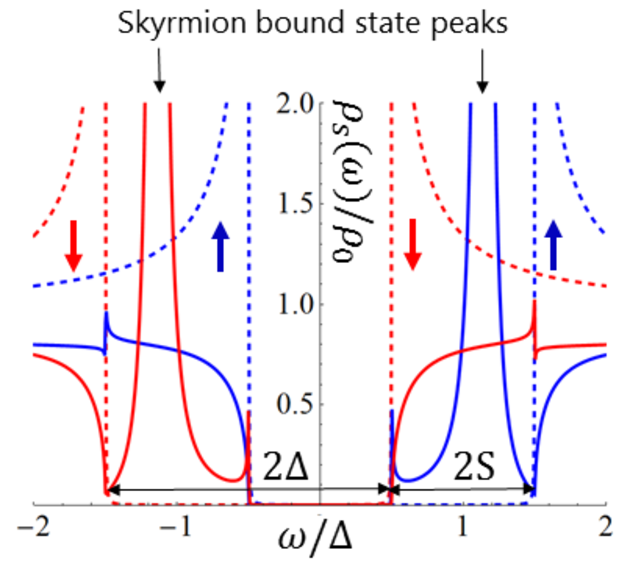
\includegraphics[width=0.7\linewidth]{fig2} 
	\caption{(Color online) Spin-polarized local density of states (SP LDOS) of SC away from the skyrmion (dashed) and at the skyrmion core (solid). The color of the curves encodes the spin polarization: blue for spin up and red for spin down as indicated by the arrows. The figure is obtained by using a model given by Eqs.~(\ref{tm1}) and (\ref{ldos}) for the parameters $2S = \Delta = 0.1 \mu$, $R = 2.5/p_F$, $S_0 = 5SR^2$, and $S_1 = 0.5 SR^3$.} \label{fig:LDOS}
\end{figure}
%%%%%%%%%%%%%%%%%%%%%%%%%%%%%%%%%%%%%%%%%%%%%%%%%%%%%%%%%%%%%%%%%%%%%%%%%%


In the current paper, we consider a FM film with a skyrmion proximity coupled to SC as shown in Fig.~\ref{fig:skyrmion}. We search for the states in SC localized around a skyrmion in a series of approximations. First we consider a limit of a small skyrmion, i.e. $R\ll \xi_{\rm sc}$, in which case we approximate the skyrmion as a point magnetic moment. Using this simplified model, we do an analytical T-matrix calculation and find that skyrmion induces a bound state in the SC in a close analogy with the well-known Yu-Shiba-Rusinov states \cite{Yu,Shiba,Rusinov,Balatsky2006}. We find that SBS induces a resonance with a finite spectral width in a spin-polarized local density of states (SP LDOS). In contrast with the conventional YSR states, which are short-range, the SBS state is a long-range state with a powerlaw decay. Therefore, in the presence of multiple skyrmions, the SC could mediate an effective long-range interaction between the skyrmions \cite{Yao2014,Shytov2009} when the SBS states overlap. Later, we relax the requirement $R\ll \xi_{sc}$ and calculate LDOS and the wavefunctions for $R\sim \xi_{sc}$ numerically. We find that the SBS peak is populated by the multiple quasilocalized states corresponding to different angular momenta. 


%%%%%%%%%%%%%%%%%%%%%%%%%%%%%%%%%%%%%%%%%%%%%%%%%%%%%%%%%%%%%%%%%%%%%%%%%%%
\paragraph*{Single skyrmion in a FM film.---} \label{sec:skyrmion}
%%%%%%%%%%%%%%%%%%%%%%%%%%%%%%%%%%%%%%%%%%%%%%%%%%%%%%%%%%%%%%%%%%%%%%%%%%


Consider a FM film with the magnetization described by a three-dimensional vector $\bm S(\bm r) = (S_x,S_y,S_z)$ dependent on a two-dimensional spatial coordinate $\bm r = (x,y)$. The topological configurations of the field $\bm S(\bm r)$ shown in Fig. \ref{fig:skyrmion}(a) and (b) are referred to as skyrmions.  Depending on a specific FM material, two distinct types of skyrmions are observed in experiment: the N\'eel (hedgehog) skyrmion and Bloch (spiral) skyrmion shown in Fig.~\ref{fig:skyrmion}(a) and (b), respectively. Although, the two types of skyrmions differ significantly in the orientation of the in-plane spins both are characterized by the same topological charge
\begin{align}
	Q = \frac{1}{4\pi} \int d^2r \, \hat {\bm S}\cdot (\nabla_x\hat {\bm S}\times\nabla_y\hat {\bm S})=1,\quad  \hat {\bm S}= \frac{\bm S}{S}. 
	\label{topCharge}
\end{align}
Thus, one can transform a Neel skyrmion into a Bloch skyrmion by a mental $\pi/2$ rotation  \footnote{\label{footnote:Rotation} Note that for the case of a spin-singlet SC given by Eq.~(\ref{ham}), the Bloch and the Neel skyrmions are equivalent since they can be related by a continuous $\pi/2$-rotation around the $z$-axis in the spin space $U = \exp(-i\pi\sigma_z/4)$. In the presence of either the spin-triplet pairing or the spin-orbit interaction, the effects of the two types of skyrmions are different.} of the FM vector around the $\hat {\bm z}$ axis in the spin space without changing a topological charge~(\ref{topCharge}). It would be intriguing to have materials that could exhibit a tunable transition between the two distinct types of skyrmions. 


%%%%%%%%%%%%%%%%%%%%%%%%%%%%%%%%%%%%%%%%%%%%%%%%%%%%%%%%%%%%%%%%%%%%%%%%%%%
\paragraph*{Superconductor proximity coupled to a ferromangetic film.--- }  \label{sec:model}
%%%%%%%%%%%%%%%%%%%%%%%%%%%%%%%%%%%%%%%%%%%%%%%%%%%%%%%%%%%%%%%%%%%%%%%%%%
Let us consider a heterostructure of a SC and FM with a skyrmion as shown in Fig.~\ref{fig:skyrmion}(a) and (b). The SC is described by the 4-by-4 Bogolyubov-de Gennes (BdG) Hamiltonian 
\begin{align}
 H &= \xi(\bm p)\tau_z+\Delta \tau_x - \bm S(\bm r)\cdot\bm\sigma, \label{ham} \\
   & \xi(\bm p) = \frac{\bm p^2}{2m}-\mu,\quad \bm p = -i(\nabla_x,\nabla_y).
\end{align}
Here, $\xi(\bm p)$ describes the kinetic energy and $\Delta$ - the self-consistent superconducting gap, which we assume uniform in space; the term $\bm S(\bm r)\cdot\bm\sigma$ describes the proximity coupling between the FM film and SC. We assume that the Zeeman splitting $S(\bm r)$ does not exceed the Chandrasekhar-Clogston limit and $S<\Delta$. The Pauli matrices $\bm \tau$ and $\bm \sigma$ act, respectively, in the particle-hole and spin subspaces of the four-component spinor $\Psi = (\psi_\uparrow,\psi_\downarrow,\psi^\dagger_\downarrow,-\psi^\dagger_\uparrow)^T$. We consider a case with a single N\'eel skyrmion \cite{Note1} centered at $\bm r = 0$, and, so, assume the following profile of the FM vector
\begin{align}
	\bm S(\bm r) &= S\left[ \cos\phi(\bm r) \sin\theta(\bm r),\, \sin\phi(\bm r)\sin\theta(\bm r),\,\cos\theta(\bm r)\right],\nonumber  \\   
	\phi(\bm r) &= \arctan(y/x),\quad \theta(\bm r) = \pi \left[ 1-\exp\left( -\frac{r^2}{R^2} \right) \right], \label{conf}	
\end{align}
where $R$ defines an effective radius of a skyrmion \footnote{We expect that a different spatial dependency of azimuthal angle (\ref{conf}) will not change the results significantly.}. Let us compare the relevant spatial scales of the problem: the SC coherence length $\xi_{\rm sc} \approx v_F/\Delta$, the skyrmion radius $R$, and the Fermi length $p_F^{-1}$. Both the scales $\xi_{\rm sc}$ and $R$ can vary from tens of nanometers to a micron depending on a specific material, whereas the Fermi length $p_F^{-1}$ is typically smaller than the other two scales. Let us first comment on the regime of the large skyrmion radius, i.e. $R\gg \xi_{\rm sc}$. In this case, the skyrmion can be viewed as a large FM domain pointing in the direction opposite to the rest of the system. Such a regime could be intriguing in the context of topological SC~\cite{Alicea2012}. For instance, it was recently shown \cite{Klinovaja2013} that a helical texture of spins in a one-dimensional (1D) chain of magnetic atoms on a surface of a SC generates an effective Rashba-like spin-orbit interaction responsible for the Majorana edge modes. Similar effective spin-orbit interaction is generated near a skyrmion and could give rise to non-trivial edge states localized at the edge of the skyrmion. We leave the discussion of this intriguing scenario to future works. In the current paper, we focus on the case of relatively small skyrmions, i.e. $R\le \xi_{sc}$. 






%%%%%%%%%%%%%%%%%%%%%%%%%%%%%%%%%%%%%%%%%%%%%%%%%%%%%%%%%%%%%%%%%%%%%%%%%%
\begin{figure} \centering
	(a)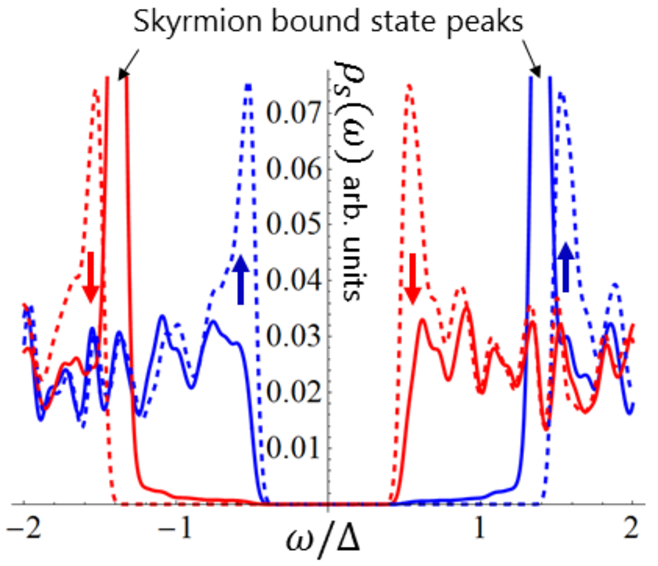
\includegraphics[width=0.7\linewidth]{fig3a} \\  
	(b)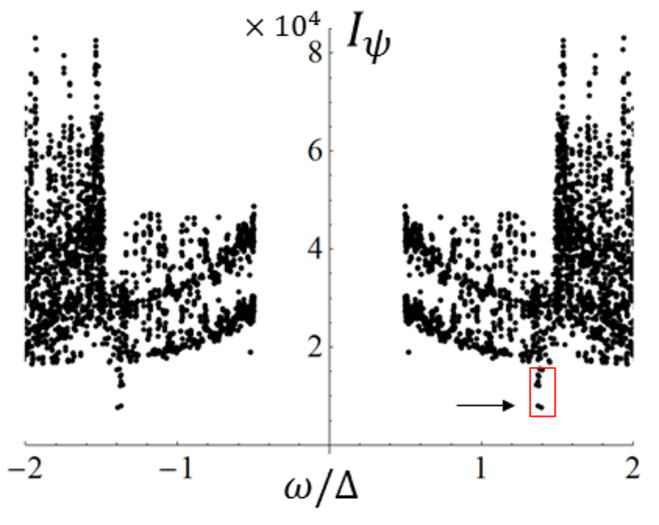
\includegraphics[width=0.7\linewidth]{fig3b} 
	\caption{(Color online) Numerical modeling of a skyrmion. (a) Spin-polarized LDOS at the skyrmion core (solid) and away from the skyrmion (dashed).  (b) Participation ratio representing a degree of localization of the BdG wavefunctions $\psi$. Few of the quasilocalized wavefunctions emphasized by the red square are shown in Fig.~\ref{fig:wavefunction}.} \label{fig:LDOSNumerics}
\end{figure}
%%%%%%%%%%%%%%%%%%%%%%%%%%%%%%%%%%%%%%%%%%%%%%%%%%%%%%%%%%%%%%%%%%%%%%%%%%


%%%%%%%%%%%%%%%%%%%%%%%%%%%%%%%%%%%%%%%%%%%%%%%%%%%%%%%%%%%%%%%%%%%%%%%%%%%
\paragraph*{Multipole expansion of the skyrmion.---} \label{sec:analytics}
%%%%%%%%%%%%%%%%%%%%%%%%%%%%%%%%%%%%%%%%%%%%%%%%%%%%%%%%%%%%%%%%%%%%%%%%%%%
Let us consider a case of a small skyrmion, i.e. $R\ll\xi_{\rm sc}$. In this limit, the SC cannot ``resolve'' the fine details of the field $\bm S(\bm r)$. We perform the multipole expansion of the skyrmion configuration~(\ref{conf}) and approximate it as a point magnetic moment floating in a ``ferromagnetic sea'' as illustrated in Fig.~\ref{fig:skyrmion}(c)
\begin{align}
	\bm S_{\rm approx}(\bm r) & =  - S \hat{\bm z} + S_0 \hat{\bm z} \delta^2(\bm r),  \label{vr}
\end{align}
where $S_0$ is the zeroth moment of $\bm S(\bm r)$ 
\begin{align}
	S_0 = \int  d^2r \, \left[\bm S(\bm r)-\bm S(\infty)\right]_z  \quad \sim \,\,\,SR^2. \label{S0} 
\end{align}
The formal domain of validity of the multipole expansion is $R \le p_F^{-1} \ll \xi_{sc}$\footnote{The domain of applicability can also be extended to $p_F^{-1}<R\ll \xi_{sc}$ with some modification of the theory.}. The multipole expansion gives an elegant and physically transparent description of the system, and, for this reason, we use it even beyond the domain of validity. In the end of the paper, we present an exact numerical modeling and find a close agreement with a multipole analytical treatment.  

By performing the T-matrix calculation, we solve the model given by Eqs.~(\ref{ham}) and (\ref{vr}), where we treat the local term $S_0 \hat{\bm z} \delta^2(\bm r)$ as a perturbation. We include the constant background magnetization $-S\hat{\bm z}$ in the BdG Hamiltonian $h(\bm p) = \xi(\bm p)\tau_z+\Delta \tau_x +  S\sigma_z$ and calculate an on-site matrix element of the bare Green's function $g(\omega,\bm p) = [\omega-h(\bm p)]^{-1}$ 
 \begin{align}
	 g_{0}(\omega)  =-\pi\rho_0\sum_{\lambda = \pm 1} \frac{1+\lambda\sigma_z}{2}\,\frac{\omega-\lambda S+\Delta\tau_x}{\sqrt{\Delta^2-\left( \omega-\lambda S \right)^2}},  \label{grf}
\end{align}
where $\rho_0 = m/2\pi$ is the density of states. This Green's function describes a SC subject to a uniform background magnetization $-\hat{\bm z} S$ that shifts the spin subbands as shown with the dashed lines in Fig.~\ref{fig:LDOS}.  The density of states contains two interior and two exterior coherence peaks at the energies $\pm(\Delta-S)$ and $\pm(\Delta+S)$ correspondingly.  Using Green's function~(\ref{grf}) we calculate the T-matrix in the presence of a point magnetic moment $V(\bm r)=S_0\,\sigma_z \delta^2(\bm r)$ representing the skyrmion
\begin{align}
	T(\omega) =   \frac{-S_0\sigma_z}{1+S_0\sigma_zg_{0}(\omega)}. \label{tm} 
\end{align}
The poles of T-matrix give the energies of the skyrmion-induced bound states (SBS)
\begin{align}
	E^\pm_{\rm SBS} = \pm\left[S+\Delta \frac{1-\left( \pi\rho S_0 \right)^2}{1+\left( \pi\rho S_0 \right)^2}\right].
	\label{energy}
\end{align}
Let us track the SBS energies as a function of increasing $S_0$, which is an implicit function of $S$ and $R$ according to Eq.~(\ref{S0}). For vanishing $S_0$, the SBS states lie at the outer coherence peaks at the energies $\pm (\Delta+S)$. With further increase of $S_0$, the SBS states split from the outer coherence peak and move to the inner coherence peaks. \footnote{Although Eq.~(\ref{energy}) suggests that the SBS states may go inside the actual gap for large enough  $S_0$, i.e. $|E^\pm_{\rm SBS}|<\Delta-S$, the multipole approximation of a skyrmion (\ref{vr}) is no-longer valid in this regime and, thus, does not give a reliable estimate of the SBS energy. In practice, by performing a numerical modeling, we never observe the SBS peaks inside the actual spectral gap, i.e. in the window of energies $|E^\pm_{\rm SBS}|<\Delta-S$.} The spin-polarization of the SBS states is determined by the spin-polarization of the bulk bands that they split from: the positive (negative) SBS state is ``up'' (``down'') spin-polarized. The SBS states closely mimic the well-known Yu-Shiba-Rusinov (YSR) states \cite{Yu,Shiba,Rusinov,Balatsky2006} localized around magnetic impurities in SC. The main difference is that the YSR energies reside inside the actual spectral gap, whereas the SBS energies lie in the window of energies $\Delta+S>|E^\pm_{\rm SBS}|>\Delta-S$, which is also filled with a continuum of delocalized states of the opposite spin polarization.  

Now let us show that SBS gives a resonance of finite spectral width due to the coupling with the continuum of delocalized states. Indeed, the skyrmion has in-plane spins at $r\approx R$ that couple the spin-up and spin-down sectors of the Hamiltonian. In order to capture this effect we append the multipole expansion (\ref{vr}) with a next order term  mimicking the radial in-plane spins of the skyrmion.
\begin{align}
	\bm S_{\rm approx}(\bm r) & =  - S \hat{\bm z} + S_0 \hat{\bm z} \delta^2(\bm r)-S_1 \bm \nabla \delta^2(\bm r), \label{vr1}
\end{align}
where  $\bm \nabla = (\nabla_x,\nabla_y)$ and $S_1$ is the first-moment of the original skyrmion configuration $\bm S(\bm r)$
\begin{align}
	S_1 = \frac{1}{2}\int  d^2r \, \left[\bm S(\bm r)-\bm S(\infty)\right] \cdot \bm r\quad \sim \,\,\,SR^3. \label{S1}
\end{align}
In Supplemental Material, we solve the Lippmann-Schwinger equation for the T-matrix and obtain
\begin{align}
	T(\omega) =   \frac{-S_0\sigma_z+S^2_1p_F^2\bar g_{0}(\omega)}{1+S_0\sigma_zg_{0}(\omega)-S^2_1p_F^2\,\bar g_{0}(\omega)\, g_{0}(\omega)}, \label{tm1} 
\end{align}
where we define the Green's function $\bar g_0(\omega) = \frac{1}{2}\sum_{j=x,y} \sigma_j g_0(\omega) \sigma_j $, which describes the bands with opposite spin polarization $\sigma_z\rightarrow -\sigma_z$. Using Eq.~(\ref{tm1}) we calculate SP LDOS 
\begin{align}
	\rho_s & (\omega) = \label{ldos} \\ 
	&-\frac{1}{\pi}\,{\rm Im}{\rm \,Tr} \left\{  \frac{1+\tau_z}{2}\,\frac{1+\sigma_s}{2} \left[g_0(\omega)+g_0(\omega) T(\omega) g_0(\omega)  \right]\right\},\nonumber 
\end{align}
where $s=x,y,z$ denotes the spin projection axis. We plot LDOS (\ref{ldos}) with solid lines in Fig.~\ref{fig:LDOS} and compare it with LDOS away from the skyrmion shown with dashed lines. We observe that the peaks corresponding to the SBS resonances have finite spectral width. Indeed, the denominator of T-matrix~(\ref{tm1}) has an extra term compared to that of Eq.~(\ref{tm}). The first two terms in the denominator of (\ref{tm1}) give the SBS energies~(\ref{energy}), whereas the last term $S^2_{\rm m}p_F^2\,\bar g_{0}(\omega)\, g_{0}(\omega)$ is imaginary and defines the spectral width of the SBS resonance observed in Fig.~\ref{fig:LDOS}. 



%%%%%%%%%%%%%%%%%%%%%%%%%%%%%%%%%%%%%%%%%%%%%%%%%%%%%%%%%%%%%%%%%%%%%%%%%%%
\paragraph*{Numerical analysis.---} \label{sec:numerics} 
%%%%%%%%%%%%%%%%%%%%%%%%%%%%%%%%%%%%%%%%%%%%%%%%%%%%%%%%%%%%%%%%%%%%%%%%%%%
So far we have analyzed a skyrmion using an analytical multipole approximation. Now let us present the results of an exact numerical modeling. We set the BdG Hamiltonian on a N-by-N tight-binding square lattice with parameters: the lateral size N = 200, nearest neighbor coupling $t$, on-site superconducting pairing and Zeeman coupling $\Delta=2S=0.1t$, and chemical potential $\mu = -3t$. This choice of parameters corresponds to $\xi_{\rm sc}\approx 17 a$ in the units of the elementary cell constant $a$. The skyrmion is described by the vector $\bm S(\bm r)$ given by Eq.~(\ref{conf}) with the effective radius $R = 6a$, so that $2R\sim \xi_{\rm sc}$. From the numerical wavefunction, we perform the Gaussian smoothing of the SP LDOS and plot it in Fig.~\ref{fig:LDOSNumerics}(a). We use the same plotting style as in Fig.~\ref{fig:LDOS}: solid (dashed) line represents LDOS at the (away from) skyrmion, whereas colors encode spin polarizations. We observe that the calculated LDOS is consistent with the results of the analytical calculation. Away from the skyrmion, SP LDOS contains the shifted spin subbands. At the skyrmion core, the skyrmion induces a strong resonance in the energy window $\Delta-S<|\omega|<\Delta+S$. In order to further analyze the numerical wavefunctions $\psi(\bm r)$, we also calculate the following expression 
\begin{equation}
	I_\psi =\frac{1}{\sum_{\bm r} |\psi(\bm r)|^4},
	\label{I}
\end{equation}
where the sum is carried over all lattice sites $\bm r$. The function $I_\psi$ gives a degree of a localization of the wavefunction $\psi(\bm r)$ \footnote{The inverse $I_\psi^{-1}$ is commonly referred to as the inverse participation ratio.}. The function is small $I_\psi \sim 1$ for an extremely localized wavefunction and large $I_\psi \sim N^2$ for a delocalized wavefunction. For each numerical BdG wavefunction $\psi(\bm r)$, we plot $I_\psi$ against the eigenenergy in Fig.~\ref{fig:LDOSNumerics}(b) and superpose it with SP LDOS shown in panel (a). To our delight, we observe a number of states that stand out distinctly from the rest of states as emphasized by the red rectangle in Fig.~\ref{fig:LDOSNumerics}(b). This states have approximately the energy of the SBS peak, and their number grows with a skyrmion size. We plot spatial profile of the electron part of the BdG wavefunction $|\Psi(\bm r)|^2 = |u_{\uparrow}(\bm r)|^2+|u_{\downarrow}(\bm r)|^2$  for a few of these states in Fig.~\ref{fig:wavefunction}. In contrast with the analytical results, we find a wavefunction with multiple lobes corresponding to a higher angular momentum state, shown in panel (a), as well as a state with a single peak, shown in panel (d).  

We also observe that all wavefunctions in Fig.~\ref{fig:wavefunction} exhibit characteristic oscillations at a scale $\xi_{\rm sc}$. In order to understand this behavior, consider a generic wavefunction of an impurity induced state ${\Psi_\lambda(\bm r) \sim e^{ip_Fr-r\sqrt{\Delta^2-\omega^2_\lambda}/v_F}/\sqrt{r}}$, where $\lambda$ denotes the eigenvalues of $\sigma_z$ operator and $\omega_\lambda = \omega - \lambda S$. The terms in the exponent term describe the fast Friedel oscillations at a scale as well as behavior at a scale of $\xi_{\rm sc}$. For clarity, let us focus the positive SBS state, i.e. $\omega = E^{+}_{\rm SBS}$. From the point of view of spin-up subband shown in blue in Fig.~\ref{fig:LDOSNumerics}(a), the SBS state is a subgap state, i.e. $\omega_+<\Delta$, and, so, the wavefunction $\Psi_+(\bm r)$ is exponentially localized. However from the point of view of spin-down subband shown in red in Fig.~\ref{fig:LDOSNumerics}(a), the SBS is a supragap state, i.e. $\omega_->\Delta$, and, so, the SBS state  $\Psi_-(\bm r)  \sim e^{ip_Fr+ir\left|\sqrt{\omega^2_--\Delta^2}\right|/v_F}/\sqrt{r}$ displays oscillations  at a scale of $\xi_{sc}$ superimposed with a long-range power law $1/\sqrt{r}$ decay. These oscillations as well the long-range behavior are visible in Fig.~\ref{fig:wavefunction}. In such a way, we show that the SBS are long-range quasilocalized states in stark contrast with the exponentially localized YSR states. 


%%%%%%%%%%%%%%%%%%%%%%%%%%%%%%%%%%%%%%%%%%%%%%%%%%%%%%%%%%%%%%%%%%%%%%%%%%
\begin{figure} \centering
	(a)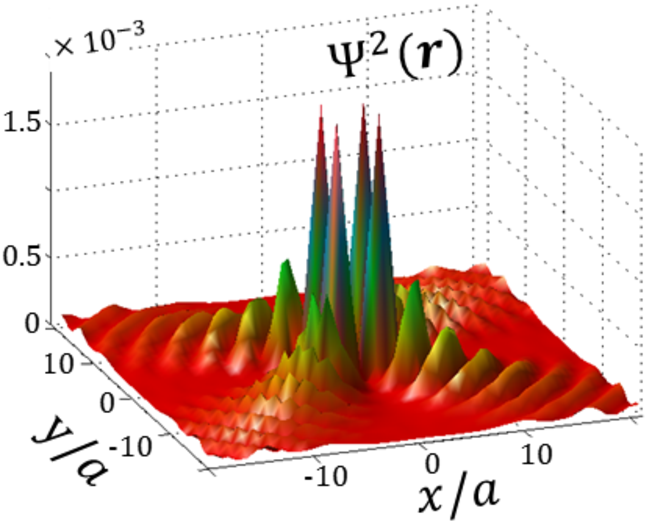
\includegraphics[width=0.43\linewidth]{fig4a}  
	(b)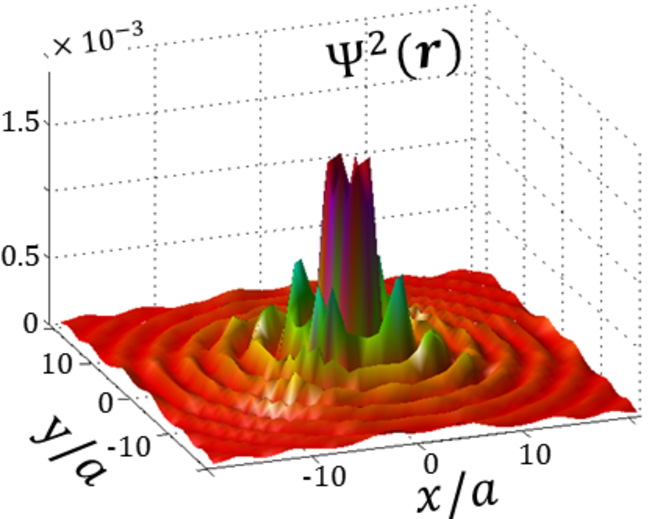
\includegraphics[width=0.43\linewidth]{fig4b} \\
	(c)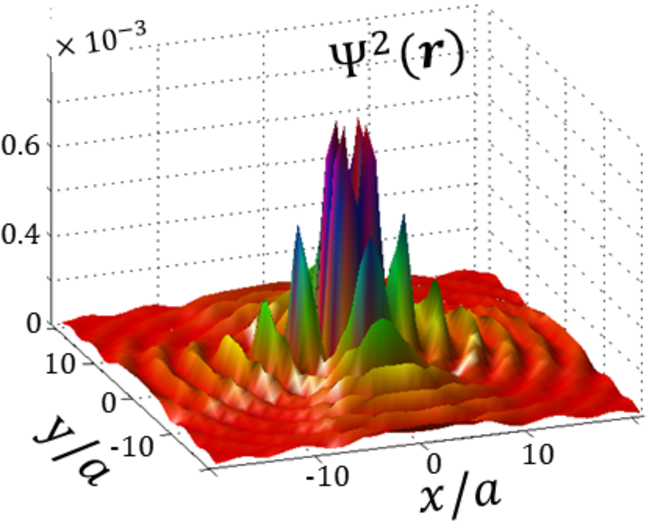
\includegraphics[width=0.43\linewidth]{fig4c}  
	(d)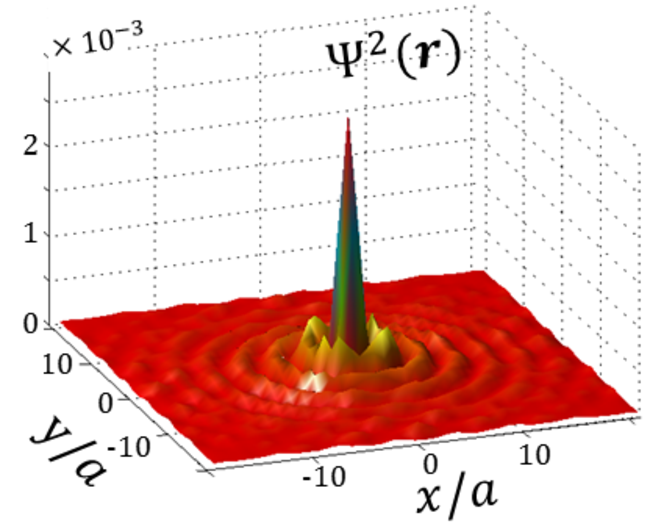
\includegraphics[width=0.43\linewidth]{fig4d} 
	 \caption{(Color online) Spatial profile of the quasilocalized wavefunctions obtained numerically, which are indicated in Fig.~\ref{fig:LDOSNumerics}(b). The wavefunctions are shown in the order of increasing $I_\psi$.  } \label{fig:wavefunction}
\end{figure}
%%%%%%%%%%%%%%%%%%%%%%%%%%%%%%%%%%%%%%%%%%%%%%%%%%%%%%%%%%%%%%%%%%%%%%%%%%




%%%%%%%%%%%%%%%%%%%%%%%%%%%%%%%%%%%%%%%%%%%%%%%%%%%%%%%%%%%%%%%%%%%%%%%%%%%
\paragraph*{Conclusion and Outlook.---} \label{sec:conclusion}
%%%%%%%%%%%%%%%%%%%%%%%%%%%%%%%%%%%%%%%%%%%%%%%%%%%%%%%%%%%%%%%%%%%%%%%%%%%

In this paper, we predict a new skyrmion bound state (SBS) in SC proximity coupled to the FM film with a skyrmion. We calculate SP LDOS and show the signatures of SBS in the tunneling spectrum that could be measured by the spin-polarized scanning tunneling microscopy (SP STM). The skyrmion typically induces a resonance in between the spin-split coherence peaks corresponding to the opposite spin polarizations. We show that the wavefunction of SBS is quasilocalized, i.e. decays as $1/\sqrt{r}$. Thus in the case of the two skyrmions, their SBS wavefunctions will overlap and induce a long-range interaction between skyrmions \cite{Yao2014,Menard2015}. The details of the long-range interaction will be explored in a subsequent publication. 

We hope that the current paper will be a first step in studying SC-skyrmionic heterostructures and motivate further research. There are intriguing questions to explore. For instance, SC could induce an effective Dzyaloshinkii-Moriya especially in non-centrosymmetric materials and, thus, stabilize the skyrmionic phase. It would also be interesting to consider the connection with the topological SC hybrid systems \cite{Alicea2012}. Superconductivity could potentially endow skyrmions with a non-trivial statistics if skyrmions captivate Majorana fermions \cite{Kim2015}. 

We thank  R.~Wiesendanger, Fujimoto, J.~Zang, A.~Saxena, H. Hurst, and Y. Tserkovnyak for valuable discussions and comments. This work was supported by the US DOE BES E304, ERC DM-321031 and KAW. 

\newpage

%%%%%%%%%%%%%%%%%%%%%%%%%%%%%%%%%%%%%%%%%%%%%%%%%%%%%%%%%%%%%%%%%%%%%%%%%%%%%
\bibliography{Skyrmion}
%%%%%%%%%%%%%%%%%%%%%%%%%%%%%%%%%%%%%%%%%%%%%%%%%%%%%%%%%%%%%%%%%%%%%%%%%%%%%


\appendix 

%%%%%%%%%%%%%%%%%%%%%%%%%%%%%%%%%%%%%%%%%%%%%%%%%%%%%%%%%%%%%%%%%%%%%%%%%%%%%
\section{T-matrix analysis} \label{sec:appendixTMatrix}
%%%%%%%%%%%%%%%%%%%%%%%%%%%%%%%%%%%%%%%%%%%%%%%%%%%%%%%%%%%%%%%%%%%%%%%%%%%%%


In this section, we provide details on the derivation of the T-matrix~(\ref{tm1}) for the model given by Eqs.~(\ref{ham}) and (\ref{vr1}).  In the momentum space, the local terms defined via the delta functions in Eq.~(\ref{vr1}) generate the following perturbation 
\begin{equation}
	V(\bm p) = -S_{\rm e}\,\sigma_z +  i \,S_{\rm m} \, \bm \sigma\cdot \bm  p.
	\label{vp}
\end{equation}
Using Eq.~(\ref{vp}) and the bare Green's function~(\ref{grf}), we write the Lippmann-Schwinger integral equation for the T-matrix
\begin{align}
	T\left(\bm p^{1},\bm p^{2}\right) &= V \left(\bm p^{1}-\bm p^{2}\right) \nonumber \\
	& +\int \frac{d^2 p'}{\left( 2\pi \right)^2}\, V\left(\bm p^{1}-\bm p'\right) g(\omega,\bm p')  T\left(\bm p',\bm p^{2}\right).
	\label{integEq}
\end{align}
Since in the case of the superconductivity we are interested in the scatterings close to the Fermi surface, we use $\bm p^{1} = p_F\, \bm n^{1}$ and $\bm p^{2} = p_F \,\bm n^{2}$, where the in-plane unit vectors $\bm n^{1}$ and $\bm n^{2}$ determine the direction of scattering on the Fermi surface.  Then, we seek the T-matrix in the following form
\begin{align}
	T\left(\bm n^{1},\bm n^{2}\right) &= A + B_i n^{1}_i + C_i n^{2}_j + D_{ij} n^{1}_i n^{2}_j, \label{ansatz}
\end{align}
where  $A,B_i,C_i$ and $D_{ij}$ are the 4-by-4 matrices in the space $\sigma\otimes\tau$. We substitute ansatz~(\ref{ansatz}) in the integral Eq.~(\ref{integEq}), solve for the unknown matrices $A,B_i,C_i,D_{ij}$ and finally obtain the T-matrix
\begin{widetext}
\begin{equation}
	T\left(\bm n^{1},\bm n^{2}\right) = \frac{-S_{\rm e}\sigma_z+S^2_{\rm m}p_F^2\bar g_{0}(\omega)+i\,S_{\rm m}\,p_F \,  \bm \sigma\cdot(\bm n^{2}- \bm n^{1}) +S^2_{\rm m}\, p^2_F \, \bar g_{0}(\omega)\,\left(\bm \sigma\cdot\bm n^{2}\right)\,\left(\bm \sigma\cdot \bm n^{1}\right)}{1+S_{\rm e}\sigma_zg_{0}-S^2_{\rm m}p_F^2\,\bar g_{0}(\omega)\, g_{0}(\omega)}. \label{TM}
\end{equation}
\end{widetext}
For brevity, $\bar g_0(\omega) = \frac{1}{2}\sum_{j=x,y} \sigma_j g_0(\omega) \sigma_j $ denotes the Green's function obtained from $g_{0}$ by replacing $\sigma_z \rightarrow - \sigma_z$. The density of states per spin is denoted as $\rho_0 = m/2\pi$. So, in the presence of the skyrmion, the Green's function becomes
\begin{align}
	G(\omega,\bm p^1,\bm p^2) =& g(\omega,\bm p^1)\,(2\pi)^2\delta(\bm p^1-\bm p^2) \nonumber \\ 
	          &  +g(\omega,\bm p^1) T(\bm p^1,\bm p^2) g(\omega,\bm p^2),
	\label{G}
\end{align}
using which the spin-polarized local density of states (LDOS) can be expressed
\begin{align}
	\rho_s(\omega,\bm r) = -&\frac{1}{\pi}\,{\rm Im}\lim_{\omega\rightarrow \omega+i\delta}{\rm\,Tr} \left[ \frac{1+\tau_z}{2}\,\frac{1+\sigma_s}{2} \right. \label{rhor} \\
	&\left.\int \frac{d^2p^1\,d^2p^2}{\left( 2\pi \right)^4} e^{i\left( \bm p^1-\bm p^2 \right)\bm r} G(\omega,\bm p^1,\bm p^2)\right]\, \nonumber 
\end{align}
where $s=x,y,z$ denotes the spin quantization axis. It can be easily evaluated for instance at the skyrmion core, i.e. at $\bm r=0$,
\begin{align}
	& \rho_s(\omega,0) = -\frac{1}{\pi}\,{\rm Im}\lim_{\omega\rightarrow \omega+i\delta}{\rm \,Tr} \left\{  \frac{1+\tau_z}{2}\,\frac{1+\sigma_s}{2}  \right. \label{spldos} \\
	&\left.\left[g_0(\omega)+g_0(\omega)  \frac{-S_{\rm e}\sigma_z+S^2_{\rm m}p_F^2\bar g_{0}(\omega)}{1+S_{\rm e}\sigma_zg_{0}(\omega)-S^2_{\rm m}p_F^2\,\bar g_{0}(\omega)\, g_{0}(\omega)} g_0(\omega)  \right]\right\}\, \nonumber 
\end{align}
which gives the expression in Eq.~(\ref{tm1}).
%%%%%%%%%%%%%%%%%%%%%%%%%%%%%%%%%%%%%%%%%%%%%%%%%%%%%%%%%%%%%%%%%%%%%%%%%%%
%\begin{figure*} \centering
%	(a)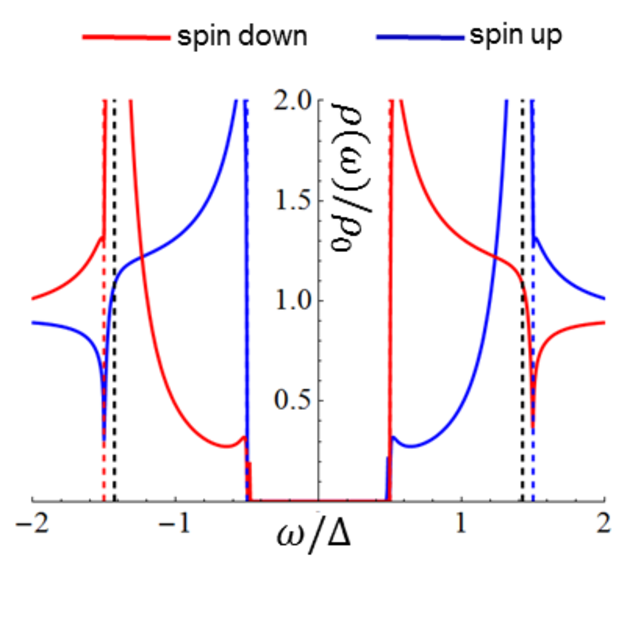
\includegraphics[width=0.25\linewidth]{ApLDOSa} \hspace{0.1cm}
%	(b)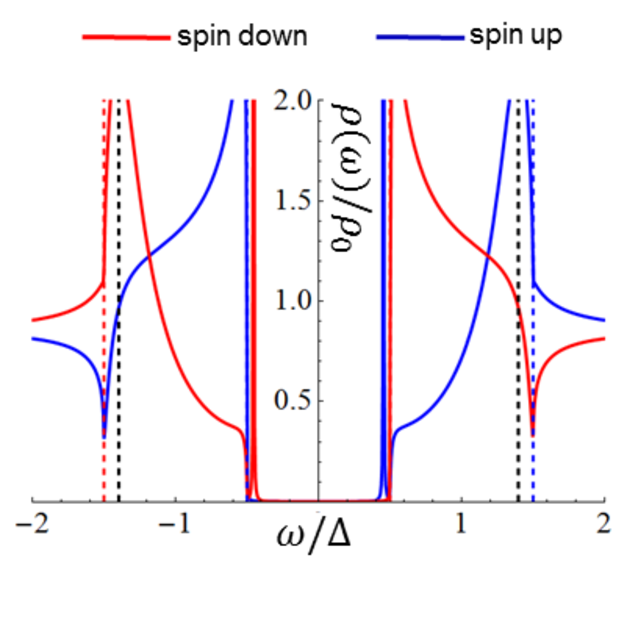
\includegraphics[width=0.25\linewidth]{ApLDOSb} \hspace{0.1cm}
%	(c)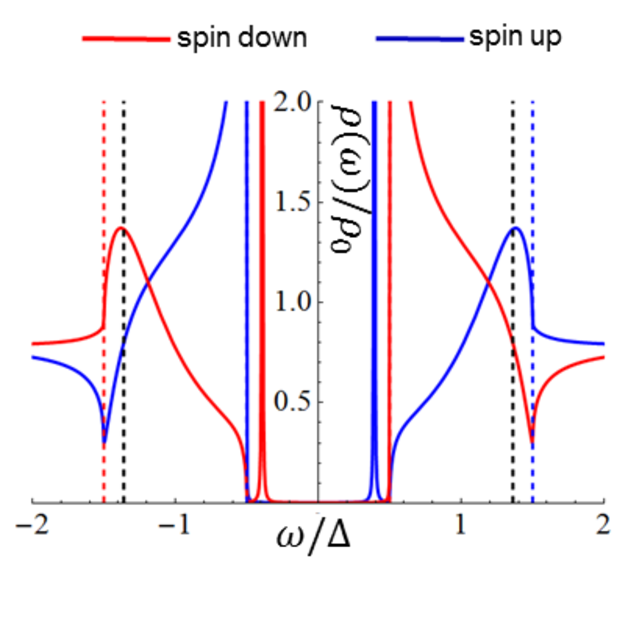
\includegraphics[width=0.25\linewidth]{ApLDOSc} 
%	\caption{(Color online) Spin-polarized local density of states (SP-LDOS)  at the core of the skyrmion. The consequent panels correspond to increasing skyrmion size (a) $R = 1.1 p_F^{-1}$, (b) $R = 1.2 p_F^{-1}$, (c) $R = 1.3 p_F^{-1}$. Other parameters are the same as in Fig.~\ref{fig:LDOS}. } \label{fig:ApLDOS}
%\end{figure*}
%%%%%%%%%%%%%%%%%%%%%%%%%%%%%%%%%%%%%%%%%%%%%%%%%%%%%%%%%%%%%%%%%%%%%%%%%%

%%%%%%%%%%%%%%%%%%%%%%%%%%%%%%%%%%%%%%%%%%%%%%%%%%%%%%%%%%%%%%%%%%%%%%%%%%%%%
%\section{Wave function of the resonance} \label{sec:wf}
%%%%%%%%%%%%%%%%%%%%%%%%%%%%%%%%%%%%%%%%%%%%%%%%%%%%%%%%%%%%%%%%%%%%%%%%%%%%%
%In this section, we discuss the wavefunction corresponding to SBS resonance. The treatment is analogous to the discussion of T-matrix in the previous setion. We write Eq.~(\ref{hbdg}) in the form of the BdG equation in the momentum space
%\begin{align}
%	\left[ \omega - h(\bm p) \right] \Psi(\bm p)= \int \frac{d^2 p'}{\left( 2\pi \right)^2}\,V(\bm p-\bm p')\,\Psi(\bm p'),	\label{bdge}
%\end{align}
%where $\Psi(\bm p)$ is the four-component wave function in the $\sigma\otimes\tau$ space. We substitute Eq.~(\ref{vp}) in the right hand side of Eq.(\ref{bdge}), use the definition of Green's function~(\ref{g}) and obtain 
%\begin{align}
%	\Psi (\bm p) = - g(\bm p) \left( S_{\rm e}\sigma_z +  i S_{\rm m}  \bm \sigma\cdot \bm  p \right)\,\Phi_1 -i\,g(\bm p)S_m\sum\limits_{j=x,y}\sigma_j \Phi_{2j},
%	\label{pwf}
%\end{align}
%where $\Phi_1$ and $\Phi_{2j}$ are the unknown four-component spinors defined self-consistently via wave function as 
%\begin{align}
%	\Phi_1 =  \int \frac{d^2 p'}{\left( 2\pi \right)^2}\, \Psi(\bm p'),\quad \Phi_{2j} =  \int \frac{d^2 p'}{\left( 2\pi \right)^2}\, p'_j\Psi(\bm p').
%	\label{f12}
%\end{align}
%Therefore, we close the equations by substituting~(\ref{pwf}) in Eq.~(\ref{f12}), take the integrals and obtain the following equations for the spinors
%\begin{align}
%	\Phi_1 &= -S_{\rm e} g_0 \sigma_z\Phi_1 - i S_{\rm m} g_{0} \sum_{j=x,y}\sigma_{j} \Phi_{2j}, \label{e1} \\
%	\Phi_{2j} &= \frac{i}{2}S_{\rm m}p_{F}^2 g_0 \sigma_j \Phi_1. \label{e2}
%\end{align}
%We substitute Eq.~(\ref{e2}) in Eq.~(\ref{e1}) and obtain the equation for $\Phi_1$
%\begin{align}
%	\left[1+S_{\rm e} g_0 \sigma_z\,\Phi_1 -  S^2_{\rm m} p_F^2\,g_{0} \bar g_{0} \right] \Psi_1 = 0. \label{le} 
%\end{align}
%This derivation is equivalent to the T-matrix treatment, and, therefore, notice that Eq.~(\ref{le}) corresponds to finding kernel of the denominator of T-matrix~(\ref{TM}). Since the matrix expression in the square brackets contains only $\sigma_z$ and $\tau_x$ matrices, the spinor $\Psi_1$  is an eigenstate of these matrices defined as ${\tau_x \mid \pm\rangle = \pm \mid \pm\rangle}$ and ${\sigma_z \mid \uparrow\downarrow\rangle = \pm \mid\uparrow\downarrow\rangle}$. That is the spinor for the positive SBS state is ${\Phi_{1} = \mid \uparrow\rangle\otimes \mid + \rangle}$ and negative - ${\Phi_{1} = \mid \downarrow\rangle\otimes \mid - \rangle}$, just as for the usual YSR state. We also substiute Eq.~(\ref{e2}) in Eq.~(\ref{pwf}) and obtain
%\begin{align}
%	\Psi(\bm p) &= - g(\bm p) \left( S_{\rm e}\sigma_z +  i S_{\rm m}  \bm \sigma\cdot \bm  p -S^2_{\rm m}p_F^2\bar g_0\right)\Phi_1,  \nonumber \\
%	&= - g(\bm p) \left( S_{\rm e}\sigma_z  - S^2_{\rm m}p_F^2\bar g_0\right)\Phi_1 -   i  S_{\rm m} g(\bm p)\,  \bm \sigma\cdot \bm  p \,\Phi_1. \label{pwf1} 	
%\end{align}
%In order to find the wave function in the real space one has to Fourier transform Eq.~(\ref{pwf1}). It can be done carefully but the resulting equations are bulky and obscure, so we are just going to show that the first term in the second line of Eq.~(\ref{pwf1}) gives exponentially localized wavefucntion, whereas the last term has a powerlaw decay and is thus long-ranged. The key element is finding the Fourier transform of the Green's function which we expand using the projector operators $(1\pm \sigma_z)/2$
%\begin{align}
%	g_{\bm r} &= \int \frac{d^2 p}{\left( 2\pi \right)^2} g(\bm p) =   \sum_{\lambda = \pm} \frac{1+\lambda\sigma_z}{2}\,g_{\bm r}^\lambda \nonumber,\quad{\rm where} \\
%	 g_{\bm r}^\lambda &=\int \frac{d^2 p}{\left( 2\pi \right)^2} \frac{e^{i\bm p \bm r}}{\omega_\lambda -\xi\tau_z-\Delta\tau_x},\,\,\omega_\lambda = \omega - \lambda S.  \label{lle}
%\end{align}
% The integral in Eq.~(\ref{lle}) can be evaluated for $r\gg v_F/\omega_D$ \cite{Pientka2013}, where $\omega_D$ is the Debye energy,
%\begin{align}
%	g^\lambda_{\bm r} = & -\pi\rho\left\{\frac{(\omega_\lambda+\Delta\tau_x)}{2\sqrt{\Delta^2-\omega_\lambda^2}}\left[ f_1(\bm r)+f_2(\bm r) \right] + \tau_x \left[ f_1(\bm r)-f_2(\bm r) \right]\right\}, \nonumber \\
%	& {\rm where}\,\,\, f_1(\bm r) = J_0\left[\left( p_F+ip_\lambda \right)r\right] + H_0\left[\left( p_F+ip_\lambda \right)r\right], \nonumber\\ 
%	& \qquad\quad f_2(\bm r) = J_0\left[\left( p_F-ip_\lambda \right)r\right] - H_0\left[\left( p_F-ip_\lambda \right)r\right], \nonumber\\
%	& \qquad\quad p_\lambda = \frac{\sqrt{\Delta^2-\omega^2_\lambda}}{v_F},
%\end{align}
%where $J_0$ and $H_0$ are the Bessel and Struve functions, $p_F$ - Fermi momentum, $p_\lambda$ characteristic momentum of a superconductor. Although the Green's function in the real space is quite bulky, it has a simple assymptotic behavior at $r\gg \xi_{sc}$
%\begin{equation}
%	g^{\lambda}_{\bm r} \sim \frac{e^{i p_F r}e^{-p_\lambda r}}{\sqrt r}. \label{asym}
%\end{equation}
%The first term describes fast Friedel oscillations, whereas second term - behavior at a scale of the superconducting coherence length $\xi_{sc}$. For the state inside the superconducting gap, i.e. for $|\omega_\lambda|<\Delta$, the latter term the exponential decay. In contrast for the state inside the continuum, i.e. for $|\omega_\lambda|>\Delta$, $p_\lambda$ becomes imaginary, i.e. $p_\lambda = -i\sqrt{\omega^2_\lambda-\Delta^2}/v_F$, and therefore the last exponential term in Eq.~(\ref{asym}) describes periodic oscillations with a period $\Delta r \sim 1/\xi_{sc}$. 

%The polarized SBS state discussed above lies inside the continuum of states corresponding to the opposite spin polarization. Moreover, the last term in Eq.~(\ref{pwf1}) describes the coupling of the state to the continuum of the background delocalized states. Thus, the SBS is expected to have an oscillating power-law rather than decaying behavior as also supported by the numerics. 

\end{document}
